\chapter{Grundlagen}
\label{sec:grundlagen}
Dieses Kapitel behandelt die für diese Arbeit nötigen Grundlagen. Zunächst wird ein Überblick über grundlegende Begriffe vorgestellt. Das Responsive Webdesign und einige Merkmale für eine responsive Webseite in Bezug auf die zu entwickelnde Webanwendung werden erläutert. Dann werden das Web 2.0 und der entstandene Ausdruck \textit{Rich Internet Application} beschrieben. Anschließend gibt es die Unterschiede zwischen Thin Client und Thick Client.

\section{Grundlegende Begriffe}
\label{sec:grundlegende begriffe}

\subsection{Workshop}
\label{sec:workshop}
Workshop\footnote{bedeutet so viel wie \glqq Arbeitskreis oder -gruppe\grqq{} .} ist eine Veranstaltung, bei der sich eine bestimmte Anzahl von Personen teilnimmt, um außerhalb der Routinearbeit Fragen, Probleme und Themen zu bearbeiten. Jeder Workshop wird von einem Moderator geleitet. Bei größeren Gruppen (mehr als 15 Teilnehmer) ist der Einsatz von weiteren Moderatoren zu empfehlen. Die Teilnehmer handeln es sich in der Regel um Spezialisten oder Betroffene, die Ihr Fachwissen zu der behandelten Aufgabe einfließen lassen. Das Ziel ist dabei: Lösungsvorschläge für Aufgaben- oder Problemstellung zu generieren und Maßnahmenplan für die Umsetzung zu entwickeln.
\\

Der Moderator ist der aktiver Dienstleister der Gruppe. Er ist für die Vorbereitung sowie Organisation verantwortlich und soll die Gruppe am Ende zum Ziel führen. Seine Aufgaben bestehen unter anderem, Fragestellung gezielt zu formulieren, den Ablaufplan zu erstellen, Denkprozesse anzuleiten, Zeitplan einzuhalten und Ergebnisse zu dokumentieren. Er muss außerdem die stille Teilnehmer aktivieren sowie die dominante bremsen und darauf achten, dass die Gruppe bei Diskussionsrunden das Ziel nicht aus den Augen verliert. 
\\

Nach Ansicht des Autors \cite{Boh2016} können Workshops in folgenden Projektphasen eingesetzt werden:

\begin{itemize} 
\item Kick-Off-Veranstaltung
\item Projektplanung-Prozess
\item Problemlösung
\item Entscheidungsfindung
\item Informationsaustausch
\item Teamentwicklung
\item Scrum
\item Projektabschluss
\end{itemize}

Die Gestaltung von Workshops spielt bei der Qualität der Ergebnisse eine große Rolle. Bei einem unstrukturierten Workshop kann dazu führen, dass er keine Motivation bei den Teilnehmer erregt, um sich an dem Workshop einzubringen und Ergebnisse zu erarbeiten. Um dagegen vorzugehen, können der Moderator je nach Dauer des Workshops folgenden kreative Workshop-Methoden anwenden, um Workshops effektiv und interaktiv zu gestalten:

\begin{itemize} 
\item World Cafe
\item Open Space
\item Six Thinking Hats
\item Fishbowl
\item Lego Serious Play
\end{itemize}

Die genauen Beschreibungen zu den oben genannten Workshop-Methoden können im Blogpost von \cite{Cho2018} verfolgt werden.
\\

Wenn es darum geht, neue Ideen für Problemlösung, neue Produkten, neue Geschäftsideen oder Innovationen zu erzeugen, werden Kreativitätstechniken eingesetzt. Denn durch Kreativität werden Ideen generiert. Viele moderne Kreativitätstechniken haben sich im Laufe der Jahre etabliert. Dem Moderator steht deshalb eine Vielzahl von Kreativitätstechniken zur Verfügung. Der Klassiker und eine der beliebtesten unter allen Kreativitätstechniken ist wie bereits im Unterkapitel \textbf{\ref{sec:motivation}} erwähnt, das klassische Brainstorming. Da die vorliegende Arbeit eine Webanwendung zur Durchführung von Workshops behandelt, die das klassische Brainstorming digitalisieren soll, werde ich deshalb nicht auf die anderen vorhandenen Kreativitätstechniken eingehen. 

\newpage
\subsection{Brainstorming}
\label{sec:brainstorming}
Wie bereits im Unterkapitel \textbf{\ref{sec:motivation}} benannt, werden beim Brainstorming anhand eines konkreten Thema bzw. Problems Ideen, Einfälle und Vorschläge gesammelt. Es kommt dabei nicht auf die Qualität der Ideen an, sondern zunächst, dass möglichst viele Ideen generiert werden. Beim Brainstorming zählt die Quantität vor Qualität. Die Teilnehmer in der Gruppe sollen ihre Gedanken öffentlich frei äußern. Durch diesen öffentlichen Austausch, können mehr Ergebnisse produziert werden.
\\

Die Gruppengröße bei einer Brainstorming-Sitzung sollte nicht zu groß und zu klein sein.  \glqq Je nach Fachliteratur ist von Gruppengröße von 5 bis maximal 20 Personen die Rede\grqq{}. \cite{Pas2012}
\\

Nach \cite{Rei2007} läuft eine Brainstorming-Sitzung in folgenden Phasen ab: 

\begin{itemize} 
\item Vorbereitung: \\
Der Moderator stellt in dieser Phase die zu behandelte Frage und die Regeln vor. Bei Notwendigkeit kann ein oder mehrere Protokollant/en bestimmt werden.

\item Ideen sammeln: \\
Die Teilnehmer dürfen Ideen und Vorschläge frei äußern. Der Moderator muss in dieser Phase vor allem die stillere Teilnehmer motivieren und ermuntern. Die Kritik ist in dieser Phase untersagt. Die Ergebnisse werden dabei protokolliert. In der Regel werden die Ideen auf eine Notizzettel geschrieben und an die Wand gepinnt.

\item Zusammenfassung und Auswertung: \\
Das Brainstorming ist nun beendet und der Moderator wird die Gruppe zunächst die dokumentierte Ergebnisse präsentieren. Anschließend werden die Ideen gemeinsam mit der Gruppe ausgewertet, sortiert und geordnet. In dieser Phase ist Kritik erlaubt und darf geäußert werden. Am Ende dieser Phase soll eine Liste mit den gut bewerteten Ideen und Vorschläge entstehen.

\item Nachbereitung: \\
Ein Brainstorming fördert nur die Kreativität. Die Vorschlägen müssen danach umgesetzt und realisiert werden. Sonst helfen die Ideen nicht, wenn nichts daraus gemacht wird.
\end{itemize}

Damit eine Brainstorming-Sitzung erfolgreich verlaufen ist, sollten dabei folgenden Regeln eingehalten werden:

\begin{itemize} 
\item Unabhängig wie verrückt jede einzelne Idee ist, keine Kritik in der Sammlungsphase.
\item Quantität vor Qualität, je mehr Ideen desto besser.
\item Entwicklung oder Verbesserung von fremden Ideen ist willkommen.
\item Lass die Fantasie freien Lauf. Ungewöhnliche Ideen sind erwünscht.
\end{itemize}

\newpage
\subsection{TCP/IP}
\label{sec:tcp/ip}
Das Transmission Control Protocol (TCP) und das Internet Protocol (IP) bilden Grundlage für die gesamte Netzwerkkommunikation und legen demnach die grundlegende Technologien für das Internet dar.
\\

TCP nutzt für die Übertragung der Datenpakete das Übertragungsprotokoll IP, welches zur Vermittlungsschicht im TCP/IP-Referenzmodell gehört. Die Aufgabe von IP-Protokoll ist, die Datenpakete an den richtigen Rechner im Netzwerk zu transportieren. Die Datenpakete sind nicht anderes als Datagramme. Ein IP-Datagramm enthält unter anderem die IP-Adresse des Absenders und des Empfängers sowie weitere spezifische Übertragungsparameter (\textbf {Abbildung \ref{fig:datagramms}}). Ob alle versendeten Datagramme erfolgreich beim Empfänger angekommen sind, kann das IP-Protokoll jedoch nicht sicherstellen. Solche Fehlerbehandlungen, wie z.B. ob Pakete beim Empfänger tatsächlich angekommen sind, stellt die Transportschicht, allem voran TCP, sicher. (vgl. \cite{Kar.o.J.}] 

\begin{figure}[H]
  \begin{center}
    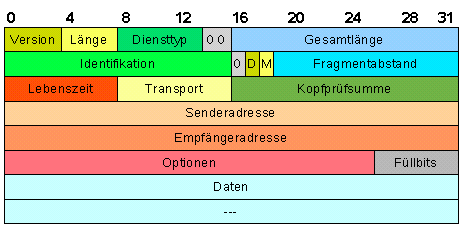
\includegraphics[width=9cm]{img/Datagramms.png}
	\caption{Aufbau eines Datagramms}
	\footnotesize\sffamily\textbf{Quelle:} \url{http://einstein.informatik.uni-oldenburg.de/rechnernetze/diagramm.htm} 
	\label{fig:datagramms}
  \end{center}   
\end{figure}

TCP ist eines der wichtigstens Protokolle der Transportschicht im TCP/IP-Referenzmodell und ist ein zuverlässiges, verbindungsorientiertes und paketvermittelndes Transportprotokoll, welches das Ziel hat, Datenverluste bei der Datenübertragung zu unterbinden, größere Datenmenge in kleinere Pakete zu zerlegen und die empfangene Datenpakete über Ports an den korrekten Anwendungen weiterzuleiten. Da sich TCP ein verbindungsorientiertes Protokoll handelt, definiert das TCP-Protokoll eine Ende-zu-Ende-Verbindung zwischen den Kommunikationspartnern im Netzwerk. (vgl. \cite{o.V.2019})
\\

Das TCP-Protokoll verwendet dabei das Verfahren namens \textit{Positive Acknowledgement (ACK) with ReTransmission\footnote{auf deutsch: positive Bestätigung mit erneuter Übertragung}}, um die Zuverlässigkeit der Datenübertragung sicherzustellen. Dies hat zu bedeuten, dass der Empfänger nach dem Erhalt der Daten dem Sender mit einer positiven Nachricht quittiert wird. Mit einer positiven Nachricht weiß der Sender, dass das Paket den Empfänger erreicht hat. Sollte von seitens der Empfänger keine positive Nachricht kommt, wird das Senden solange wiederholt, bis eine positive Antwort beim Sender eingegangen ist (\textbf {Abbildung \ref{fig:acknowledgement}}). (vgl. \cite{Hol2001})

\begin{figure}[H]
  \begin{center}
    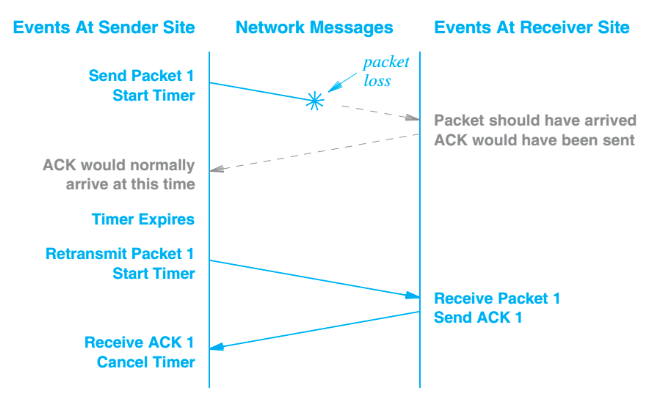
\includegraphics[width=9cm]{img/Acknowledgement.png}
	\caption{Zeitüberschreitung und erneute Übertragung bei Verlust eines Pakets}
	\footnotesize\sffamily\textbf{Quelle:} \url{http://lemoncisco.blogspot.com/2014/06/internetworking-with-tcpip-notes_25.html} 
	\label{fig:acknowledgement}
  \end{center}   
\end{figure}

Die folgende Abbildung (\textbf {Abbildung \ref{fig:tcp}}) zeigt die wichtigsten Protokolle im TCP/IP-Referenzmodell. Über der TCP- und IP-Schicht im TCP/IP-Referenzmodell befindet sich die Anwendungsschicht. Diese Schicht beinhaltet alle Protokolle auf Anwendungsebene, die auf TCP oder UDP aufsetzen. Die Anwendungsschicht stellt den Anwendungsprogrammen Dienste zur Verfügung. Das bekannteste Protokoll auf der Anwendungsschicht ist wohl das Hypertext Transfer Protocol (HTTP), welches den Zugriff auf die Webseiten ermöglicht.

\begin{figure}[H]
  \begin{center}
    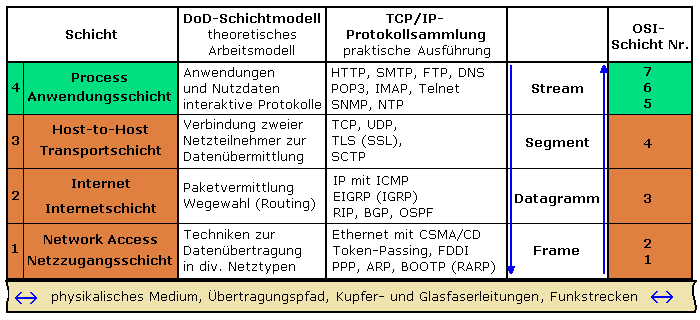
\includegraphics[scale=0.5]{img/tcp.png}
	\caption{Die wichtigsten Protokolle im TCP/IP-Referenzmodell}
	\footnotesize\sffamily\textbf{Quelle:} \url{https://www.elektroniktutor.de/internet/tcpip.html} 
	\label{fig:tcp}
  \end{center}   
\end{figure}

\newpage
\subsection{HTTP}
\label{sec:http}
Das Hypertext Transfer Protocol (HTTP) ist ein zustandsloses und unidirektionales Datenübertragungsprotokoll in einem Netzwerk. Es wird hauptsächlich eingesetzt, um die Dateien vom Server anzufordern und sie in den Browser zu laden und darzustellen. Bei HTTP handelt es sich um eine unverschlüsselte Kommunikation. Dies hat zur Folge, dass alle Informationen im Klartext gesendet werden. Für die verschlüsselte Verbindung bietet sich das sichere HyperText-Übertragungsprotokoll HTTPS\footnote{Hypertext Transfer Protocol Secure} an. HTTP arbeitet nach dem Client-Server-Modell (\textbf {Abbildung \ref{fig:client-server-modell}}). 

\begin{figure}[H]
  \begin{center}
    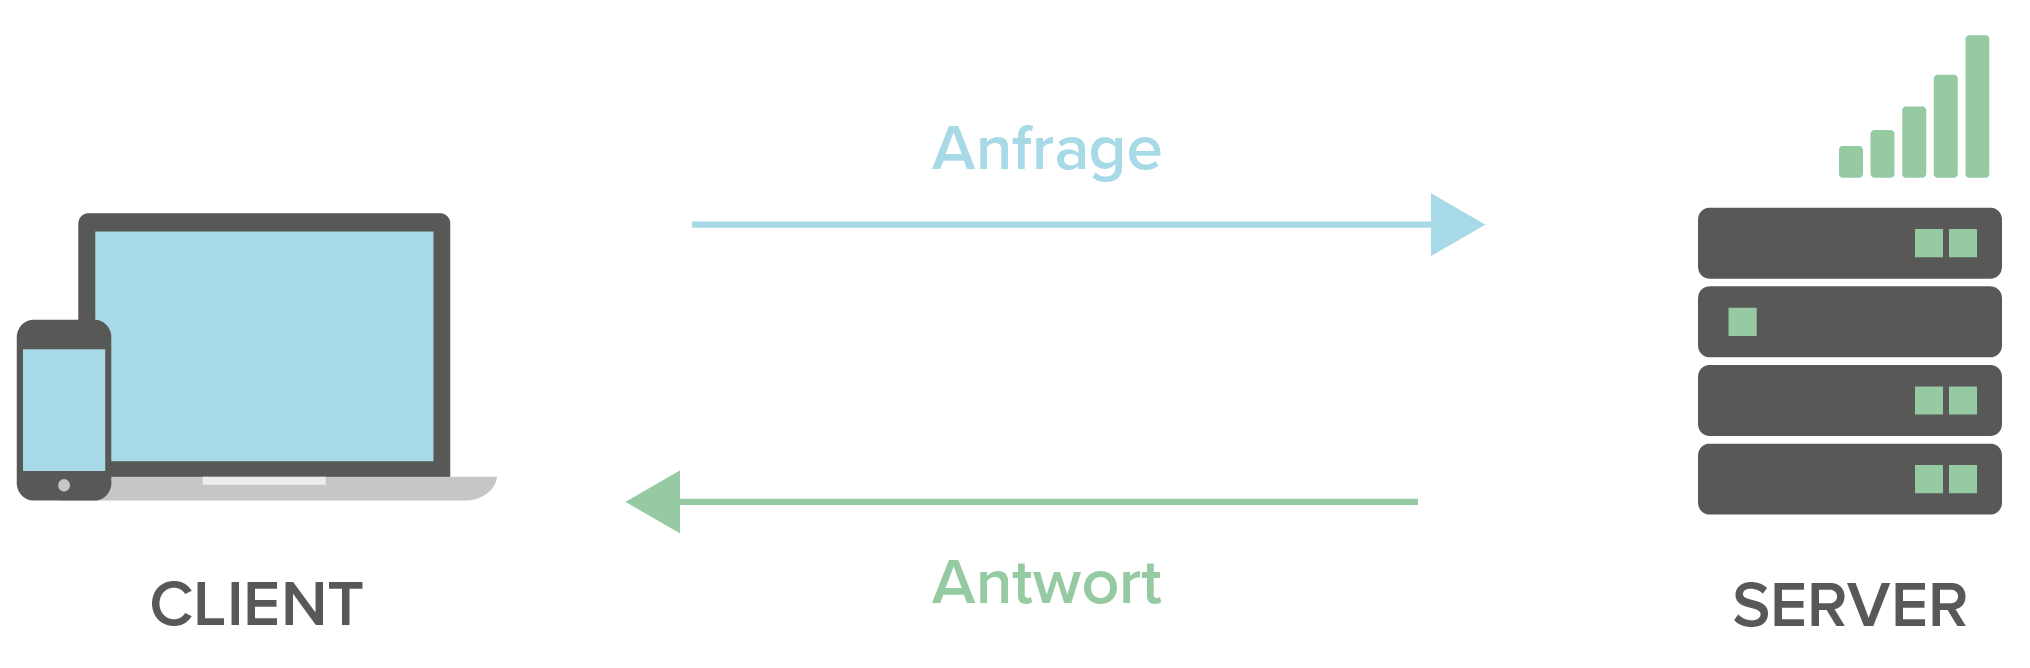
\includegraphics[scale=0.4]{img/client-server-modell.png}
	\caption{Das Client-Server-Modell}
	\footnotesize\sffamily\textbf{Quelle:} \url{https://www.placetel.de/ratgeber/client} 
	\label{fig:client-server-modell}
  \end{center}   
\end{figure}

Der Client (Webbrowser) sendet eine HTTP-Anfrage an den Port 80 des Servers (HTTP-Server). Dieser erledigt die Anfrage vom Client und schickt ihm eine Antwort zurück. Diese Kommunikation verläuft im Textformat. Die Anfrage- sowie die Antwortnachrichten bestehen aus einem Header und Daten. Der Header beinhaltet Steuerinformationen. Der Datenteil enthält den eigentlichen Inhalt der Seite. Nach Abarbeitung der Anfrage wird die Verbindung zwischen Client und Server abgeschlossen. Der Server steht also für die Bearbeitung von neuen Anfragen zur Verfügung. Um dem Server mitzuteilen, was er genau dem Client schicken soll, adressiert der Client bei der Anfrage eine Datei, die sich auf dem Server befindet muss. Dazu verwendet der Client eine URL\footnote{Uniform Resource Locator}. Ist diese Datei vom Client nicht vorhanden, antwortet der Server mit der Fehlermeldung (Error 404) zurück. Für eine zuverlässige Kommunikation verwendet HTTP das verbindungsorientierte Transportprotokoll TCP. (vgl. \cite{Lub2018})

\newpage
Eine URL ist wie folgt aufgebaut\footnote{vgl. \url{https://webdesigneinfuehrung.wordpress.com/tag-8/wie-ist-eine-url-aufgebaut/}}:

\begin{figure}[H]
  \begin{center}
    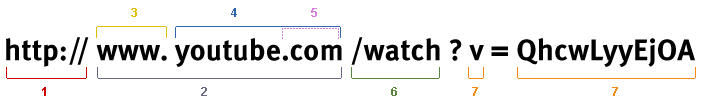
\includegraphics[scale=0.5]{img/url-aufbau.jpg}
	\caption{Aufbau einer URL}
	\footnotesize\sffamily\textbf{Quelle:} \url{https://webdesigneinfuehrung.files.wordpress.com/2013/10/url-aufbau.jpg} 
	\label{fig:url-aufbau}
  \end{center}   
\end{figure}

\begin{enumerate}
\item Das verwendete Protokoll (HTTP). Andere Protokolle könnten ebenfalls verwendet werden, wie HTTPS, FTP.
\item Es handelt sich um der Host oder Hostnamen.
\item Die Subdomain: www (World Wide Web).
\item Die Domain oder der Domainname. Dieser Name ist einmalig wie eine Postanschrift.
\item beschreibt die Top-Level-Domain und bezieht sich auf das Ursprungsland der Webseite.
\item Der Pfad. Dieser verweist auf eine bestimmte Ressource (Datei, Verzeichnis) auf dem Server.
\item Parameter und Wert: v (Parameter), QhcwLyyEjOA (Wert).\\
Nach dem Pfad folgt in dem Beispiel ein URL-Parameter. Er wird durch ein Fragezeichen getrennt.
\end{enumerate}

\subsection{Ablauf einer HTTP-Verbindung}
\label{sec:ablauf einer http-verbindung}
Der Ablauf einer HTTP-Verbindung wird mit dem Beispiel eines Aufrufes einer Webseite im Webbrowser dargestellt. Das Aufrufen einer Webseite im Browser erfolgt hauptsächlich in vier Schritten:

\begin{figure}[H]
  \begin{center}
    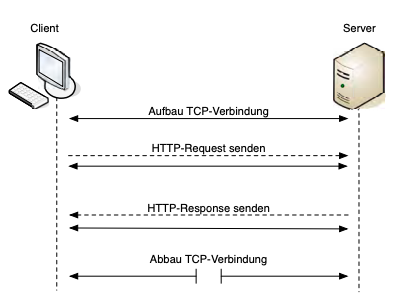
\includegraphics[scale=0.5]{img/http-request-response}
	\caption{Klassisches HTTP Request-Response-Paradigma nach \cite{Wöhr2004}}
	\label{fig:http-request-response}
  \end{center}   
\end{figure}

\newpage
\begin{enumerate}
\item Der Client baut eine TCP-Verbindung zum Server auf.
\item Der Client, in diesem Fall der Benutzer gibt z.B. eine Adresse (URL) in das Adressfeld seines Webbrowsers ein. Diese Adresse wird als HTTP-Request an der Server gesendet.
\item Der Server bearbeitet die Anfrage von dem Benutzer (Client) und antwortet ihm mit einer HTTP-Response zurück.
\item Nach dem Response baut der Server die Verbindung wieder ab.
\end{enumerate}

\subsection{AJAX}
\label{sec:ajax}
AJAX\footnote{Asynchronous JavaScript and XML} ermöglicht, dass die Daten zwischen Browser und Server im Hintergrund austauschen können, ohne die Seite komplett neu zu laden. Man spricht von einer asynchrone Datenübertragung zwischen Client und Server.
\\

Dabei ist das XMLHttpRequest\footnote{kurz: XHR}-Objekt in JavaScript für die Durchführung dieser asynchrone Datenübertragung zwischen Client und Server verantwortlich. XHR ist eine Schnittstelle zwischen JavaScript und Daten auf dem Server. Das XMLHttpRequest sendet eine HTTP-Anfrage an einen Webserver. Die Rückgabe vom Server kann ein JavaScript direkt per DOM\footnote{Document Object Modal} und CSS\footnote{Cascading Style Sheets} in das Dokument ergänzen oder verändert, ohne die Seite neu laden zu müssen. Die statische Inhalte bleiben erhalten, während nur veränderliche Information ergänzt werden. Das spart vor allem Zeit, reduziert den Trafficverbrauch und ermöglicht Nutzer interaktiv mit dem Server zu kommunizieren.
\\

Nach \cite{o.V.2017} unterstützt XHR neben XML-Dokumente auch alle Textformate und kann eine Anfrage ebenfalls über HTTPS übermitteln.
Ein typisches Beispiel für die AJAX-Anwendung ist die Autovervollständigung von Google. Sobald der Nutzer die Daten im Suchfeld auf der Google Webseite eingibt, wird dabei automatisch die passende Vorschläge geliefert. 

\begin{figure}[H]
  \begin{center}
    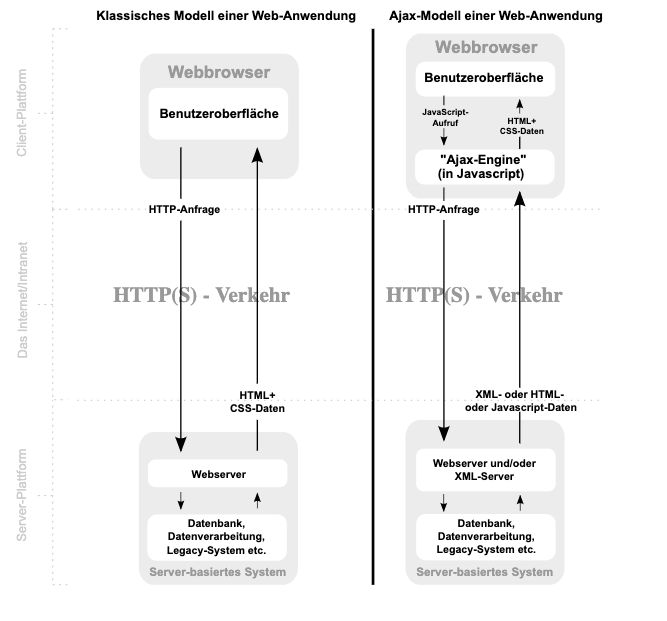
\includegraphics[scale=0.4]{img/ajax-modell}
	\caption{synchrone und asynchrone Kommunikation}
	\footnotesize\sffamily\textbf{Quelle:} By I, DanielSHaischt, CC BY-SA 3.0, https://commons.wikimedia.org/w/index.php?curid=2223689 
	\label{fig:ajax-modell}
  \end{center}   
\end{figure}

\subsection{Echtzeit}
\label{sec:echtzeit}